%%% The main file. It contains definitions of basic parameters and includes all other parts.

%% Settings for single-side (simplex) printing
% Margins: left 40mm, right 25mm, top and bottom 25mm
% (but beware, LaTeX adds 1in implicitly)
\documentclass[12pt,a4paper]{report}
\setlength\textwidth{145mm}
\setlength\textheight{247mm}
\setlength\oddsidemargin{15mm}
\setlength\evensidemargin{15mm}
\setlength\topmargin{0mm}
\setlength\headsep{0mm}
\setlength\headheight{0mm}
% \openright makes the following text appear on a right-hand page
\let\openright=\clearpage

%% Settings for two-sided (duplex) printing
% \documentclass[12pt,a4paper,twoside,openright]{report}
% \setlength\textwidth{145mm}
% \setlength\textheight{247mm}
% \setlength\oddsidemargin{14.2mm}
% \setlength\evensidemargin{0mm}
% \setlength\topmargin{0mm}
% \setlength\headsep{0mm}
% \setlength\headheight{0mm}
% \let\openright=\cleardoublepage

%% Generate PDF/A-2u
\usepackage[a-2u]{pdfx}

%% Character encoding: usually latin2, cp1250 or utf8:
\usepackage[utf8]{inputenc}

%% Prefer Latin Modern fonts
\usepackage{lmodern}

%% Further useful packages (included in most LaTeX distributions)
\usepackage{amsmath}        % extensions for typesetting of math
\usepackage{amsfonts}       % math fonts
\usepackage{amsthm}         % theorems, definitions, etc.
\usepackage{bbding}         % various symbols (squares, asterisks, scissors, ...)
\usepackage{bm}             % boldface symbols (\bm)
\usepackage{graphicx}       % embedding of pictures
\usepackage{fancyvrb}       % improved verbatim environment
\usepackage{natbib}         % citation style AUTHOR (YEAR), or AUTHOR [NUMBER]
\usepackage[nottoc]{tocbibind} % makes sure that bibliography and the lists
			    % of figures/tables are included in the table
			    % of contents
\usepackage{dcolumn}        % improved alignment of table columns
\usepackage{booktabs}       % improved horizontal lines in tables
\usepackage{paralist}       % improved enumerate and itemize
\usepackage[usenames]{xcolor}  % typesetting in color

% custom packages
\usepackage{pgfplots} % plots
\usepackage{dirtree}

%%% Basic information on the thesis

% Thesis title in English (exactly as in the formal assignment)
\def\ThesisTitle{Suggester implementation for the OpenGrok search engine}

% Author of the thesis
\def\ThesisAuthor{Bc. Adam Hornáček}

% Year when the thesis is submitted
\def\YearSubmitted{2018}

% Name of the department or institute, where the work was officially assigned
% (according to the Organizational Structure of MFF UK in English,
% or a full name of a department outside MFF)
\def\Department{Network and Labs Management Center}

% Is it a department (katedra), or an institute (ústav)?
\def\DeptType{Institute}

% Thesis supervisor: name, surname and titles
\def\Supervisor{Mgr. Vladimír Kotal}

% Supervisor's department (again according to Organizational structure of MFF)
\def\SupervisorsDepartment{Network and Labs Management Center}

% Study programme and specialization
\def\StudyProgramme{Computer Science}
\def\StudyBranch{Software and Data Engineering}

% An optional dedication: you can thank whomever you wish (your supervisor,
% consultant, a person who lent the software, etc.)
\def\Dedication{%
I would like to thank my supervisor, Mgr. Vladimír Kotal, for the opportunity to work on the OpenGrok project and for
his guidance and useful advice. I also thank my family for their support during my studies.
}

% Abstract (recommended length around 80-200 words; this is not a copy of your thesis assignment!)
\def\Abstract{%
The suggester functionality is an important feature of modern search engines. The aim of the thesis is to implement
it for the OpenGrok project. OpenGrok search engine is based on Apache Lucene and supports its query syntax.
Presented suggester implementation supports this query syntax and provides suggestions not only for the prefixes but
also for wildcards, regular expressions, or phrases. The implementation also takes into account the possibility of
grouping queries. That means, if one query is already specified and user is typing another query, then the first
query will restrict the suggestions for the second query. The promotion of specific suggestions is based on the
underlying Lucene index data structure and most popular completion.
}

% 3 to 5 keywords (recommended), each enclosed in curly braces
\def\Keywords{%
{autocomplete} {suggester} {OpenGrok} {index} {Lucene}
}

%% The hyperref package for clickable links in PDF and also for storing
%% metadata to PDF (including the table of contents).
%% Most settings are pre-set by the pdfx package.
\hypersetup{unicode}
\hypersetup{breaklinks=true}

% Definitions of macros (see description inside)
\include{macros}

% Title page and various mandatory informational pages
\begin{document}
\include{title}

%%% A page with automatically generated table of contents of the master thesis

\tableofcontents

%%% Each chapter is kept in a separate file
\chapter*{Introduction}
\addcontentsline{toc}{chapter}{Introduction}

Internet has become an unavoidable component of everyday life of billions of people. Among other things, it serves as a
source of knowledge which is available literally at our fingertips. However, it is not possible for a single person to
filter or find relevant information from such a huge dataset. As a result, many search engines emerged which try to
provide this functionality. Sometimes, users do not know for what they are exactly looking or the search engine can
predict for what the user could be looking based on some criteria. These criteria consist mainly of what the user
already typed into the system or the user's search history. Nevertheless; many others may be integrated as well, e.g.
the system can better predict search based on some personal information about the user (age, gender, etc.) or
searches of other users.


Suggester, or autocomplete, functionality tries to achieve this deficiency by giving the user the possibility to choose
from a handful of choices it deemed the most attractive for the user. Therefore, suggester implementations were added to
many search engines (e.g. Google\footnote{\url{http://google.com}}). However, OpenGrok\footnote{\url{http://opengrok.org}}
search engine does not contain any suggester implementation.

\section{Target of the thesis}

The thesis aims to fulfill the following targets:
\begin{itemize}
    \item Integrate suggester functionality into OpenGrok.
    \item Suggestions provided by the suggester should be meaningful and helpful.
    \item The suggester should provide support for rich configuration.
    \item Evaluate the impact of the suggester on the system running the OpenGrok instance.
    \item Evaluate if and how OpenGrok usage changed, that includes:
    \begin{itemize}
        \item Evaluation of the suggester usage.
        \item Evaluation of search results.
    \end{itemize}
\end{itemize}

\section{Structure}

Chapter \ref{chap:opengrok} \textbf{OpenGrok} provides a quick overview of OpenGrok project. What tools it uses and what
makes the OpenGrok project extraordinary.

Chapter \ref{chap:analysis} \textbf{Analysis} discusses problems that arose during the implementation process and how
they were resolved.

Chapter \ref{chap:user} \textbf{User Documentation} contains pictures of the added functionality and explains how it
should be used.

Chapter \ref{chap:program} \textbf{Program Documentation} describes implementation-specific properties of the work.
In other words, how exactly was the new content integrated into the OpenGrok project.

Chapter \ref{chap:impact} \textbf{Impact on the OpenGrok Project} provides detailed description, comparison and
evaluation of the functionality that affected the OpenGrok project.

% Chapter \ref{chap:epilog} % TODO: conclusion has no number so this does not work properly
% \textbf{Conclusion} concludes the work done and lists possible future extensions or enhancementes.

\chapter{OpenGrok}
\label{chap:opengrok}

\section{Overview}
\label{opengrok_overview}
OpenGrok is an open-source search engine written in
Java\footnote{\url{https://en.wikipedia.org/wiki/Java\_(programming\_language)}}
freely available at \url{https://github.com/oracle/opengrok} under CDDL
license\footnote{\url{https://en.wikipedia.org/wiki/Common\_Development\_and\_Distribution\_License}}.
However, OpenGrok is different to most of the search engines which purpose is to traverse web and find the most relevant
webpages. OpenGrok provides searching across codebases. For instance, if you would like to know which files are using
\textit{mmap} function in \textit{Linux kernel}\footnote{\url{https://en.wikipedia.org/wiki/Linux\_kernel}} then
OpenGrok is the tool for that purpose. It understands a variety of
programming languages, e.g. Java, C, C\#, JavaScript and many others. The code analysis is done by
Ctags\footnote{\url{https://en.wikipedia.org/wiki/Ctags}}.
The other most notable features of OpenGrok are:
\begin{itemize}
    \item Support for multiple projects.
    \item Support for authentization and authorization (\cite{OpengrokAuthLayer}). For instance, by using LDAP
        \footnote{\url{https://en.wikipedia.org/wiki/Lightweight_Directory_Access_Protocol}}.
    \item Support for multiple version control systems\footnote{\url{https://en.wikipedia.org/wiki/Version\_control}},
        e.g. git, mercurial, etc.
        \begin{itemize}
            \item Support for searching in repository history.
            \item Possibility to annotate a file.
            \item Possibility to see history for a specific file.
        \end{itemize}
    \item Support for cross-referencing.
    \item Support for navigation in source files. For instance, by providing list of methods.
    \item Syntax highlighting of source files.
\end{itemize}

\section{Modules}
\label{opengrok_modules}

OpenGrok is split into multiple modules:
\begin{itemize}
    \item jrcs – Java library which provides support for RCS\footnote{\url{https://en.wikipedia.org/wiki/Revision\_Control\_System}}
    version control system.
    \item Indexer – described in \ref{indexer}.
    \item Web – described in \ref{opengrok-web}.
    \item plugins – contains authorization plugins.
    \item distribution – does not contain any code and serves for combining all of the above into one distribution unit.
\end{itemize}

Visualization of these modules and how they are dependent on each other can be seen on figure \ref{opengrok_modules_img}.
\begin{figure}[htbp]
\centering
\includegraphics[width=100mm]{../img/opengrok_modules.pdf}
\caption{OpenGrok modules}
\label{opengrok_modules_img}
\end{figure}

Multiple modules support in one project is achieved by Maven\footnote{\url{https://maven.apache.org}} build tool.
There is one main \textit{pom.xml} in the root of the project which aggregates all the modules.

\subsection{Indexer}
\label{indexer}

Indexer is a submodule which main purpose is for each project to:
\begin{itemize}
    \item Generate main lookup index. Detailed description in \ref{indexer:index}.
    \item Generate history index for repositories. Detailed description in \ref{indexer:history}.
    \item Generate xref. Detailed description in \ref{indexer:xref}.
\end{itemize}

\subsubsection{Index}
\label{indexer:index}

OpenGrok heavily relies on Apache Lucene\footnote{\url{https://lucene.apache.org}}, a search engine library
written in Java. Every source file is considered to be a \textit{document}. Every \textit{document} has multiple
\textit{field}s which contain text data. This text data is then tokenized by specific rules (e.g. remove stop words,
stemming, etc.) into tokens. In the Lucene context \textit{term} is a pair of \textit{field} and \textit{token}.
Lucene uses \textit{reverse document index}\footnote{\url{https://en.wikipedia.org/wiki/Inverted_index}},
i.e. for each term a collection of document identifiers is stored in which this term occurrs.
This form of data representation is very efficient for document lookup.

\paragraph{Tokenization}
% TODO: should be here?

\paragraph{Lucene internals}
% TODO: rewrite this? http://lucene.apache.org/core/7_3_1/core/org/apache/lucene/codecs/lucene50/Lucene50PostingsFormat.html

\subsubsection{History}
\label{indexer:history}

OpenGrok uses history index for quick access to history information of every file in a project. OpenGrok first discovers
what kind of version control system the project is using and then executes appropriate commands to retrieve the project's
history (e.g. some form of \textit{git log}). Since executing these commands is not very efficient (new process has to
be created), OpenGrok does this at the indexing phase to provide better performance later. Serialized form of Java object
is stored for each source file of the project to represent its history.

\subsubsection{Xref}
\label{indexer:xref}

Main purpose of the OpenGrok is to find relevant documents based on the search query. After the successful search, the most
obvious route of action is to look at the found documents. However, analyzing the document once again, performing syntax
highlighting and other operations can be very time consuming. Therefore, \textit{xref} directory contains pre-generated
HTML\footnote{\url{https://en.wikipedia.org/wiki/HTML}} versions of every source file which already contain the
aforementioned information.

\subsection{Web}
\label{opengrok-web}

The previous section \ref{indexer:index} describes how the data are processed to create index. However, these data need
to be presented to the end user. Web submodule serves exactly this purpose. It is distributed as a
WAR\footnote{\url{https://en.wikipedia.org/wiki/WAR\_(file\_format)}} which can be used by many
servlet containers\footnote{\url{https://en.wikipedia.org/wiki/Web\_container}}. OpenGrok correctly runs in
Apache Tomcat\footnote{\url{http://tomcat.apache.org}}; nevertheless, there is no Tomcat vendor lock-in; therefore,
other servlet containers should work properly as well.

\subsubsection{Configuration}
\label{opengrok_configuration}

Since OpenGrok has two modules (Indexer and Web) which can be run separately, it needs a way how to pass relevant
information between those. However, it might be possible that Indexer finished its work after a long period of time
(in some cases it might take days) and the Web module is not reachable. Therefore, to not lose all of the information
needed by Web module the Indexer stores it as a read-only configuration. It is stored as an
XML\footnote{\url{https://en.wikipedia.org/wiki/XML}} encoded class which needs to be read by Web on its startup.
If Web module does not find the configuration on the expected place (can be configured in \textit{web.xml}) then an
error is shown on the main page and the usage is not possible. Of course, there are ways how to change the configuration
of the running OpenGrok application via the REST API \footnote{\url{https://en.wikipedia.org/wiki/Representational\_state\_transfer}}
described in the \ref{opengrok_rest}.

\subsubsection{REST API}
\label{opengrok_rest}

Opengrok provides REST API support. This is a relatively new feature. Before that, OpenGrok has known a concept of
\textit{Messages} – custom serialization of Java objects passed to Web application via custom port.
So far most of the REST API calls can be only made from the machine on which the OpenGrok runs.
This is mainly because these REST API calls are meant as a means of communication between Indexer and Web application
or for administrators maintaining the OpenGrok instance. More information can be found at
\url{https://github.com/oracle/opengrok/wiki/Web-services}.

\section{Usage}
\label{opengrok_usage}
The main purpose of the OpenGrok project is to provide ability to search codebases of software projects. This is done
mainly through its web interface. The main OpenGrok page can be seen on the figure \ref{opengrok_main}.

\begin{figure}[htbp]
    \centering
    \includegraphics[width=145mm]{../img/opengrok_main.png}
    \caption{Main OpenGrok page}
    \label{opengrok_main}
\end{figure}

The numbers in the figure \ref{opengrok_main} signify:
\begin{enumerate}
    \item Field where projects can be selected.
    \item Selected projects.
    \item Search fields.
       \begin{itemize}
        \item \textbf{Full search} – specifies the text the document should contain. Represents \textit{full} field in
        underlying Lucene implementation.
        \item \textbf{Definition} – specifies the definition of which symbol the document should contain.
        Represents \textit{defs} field in underlying Lucene implementation.
        \item \textbf{Symbol} – specifies the symbol the document should contain.
        Represents \textit{refs} field in underlying Lucene implementation.
        \item \textbf{File Path} – specifies the path the document should have.
        Represents \textit{path} field in underlying Lucene implementation.
        \item \textbf{History} – specifies the history the document should have.
        Represents \textit{hist} field in underlying Lucene implementation.
        \item \textbf{Type} – restricts the search for documents of the type.
        Represents \textit{type} field in underlying Lucene implementation.
       \end{itemize}
    \item Repository list.
\end{enumerate}

It is possible to add values to multiple search fields to make the search more specific. Into the search fields can be
typed any query written in Lucene syntax.

More detailed information with examples can be found on \textit{/help.jsp} web page of the running OpenGrok Web application instance.

\subsection{Navigating results}

\subsection{Traversing source code}

\section{Similar Tools}
It is hard to compare because all of these tools are complex and each of them provides unique feel and solution to problems.
Therefore, the list will only mention if those tools contain suggester functionality. Still, this might not be the best
indicator because they might provide different solutions, e.g. instant search which might make the suggester a redundant asset.
List of similar tools:
\begin{itemize}
    \item \textbf{SourceGraph} \url{https://about.sourcegraph.com} – SourceGraph does support instant search feature.
    While writing some text to the search field it immediately displays the files in which the text was found. The figure
    \ref{sourcegraph} shows how this feature looks like.

    \begin{figure}[htbp]
        \centering
        \includegraphics[width=145mm]{../img/sourcegraph.png}
        \caption{SourceGraph instant search feature}
        \label{sourcegraph}
    \end{figure}

    \item \textbf{searchcode} \url{https://searchcode.com/} – it seems that searchcode does not support neither
    autocomplete or instant search feature.

    \item \textbf{livegrep} \url{https://livegrep.com/} – supports instant search. Immediately shows files and their contents
    where the text was found. The look of this application can be seen on figure \ref{livegrep}.

    \begin{figure}[htbp]
        \centering
        \includegraphics[width=145mm]{../img/livegrep.png}
        \caption{livegrep instant search feature}
        \label{livegrep}
    \end{figure}

\end{itemize}

\chapter{Title of the second chapter}

\section{Title of the first subchapter of the second chapter}

\cite{Mihov01directconstruction}

\section{Title of the second subchapter of the second chapter}

\chapter{User Documentation}
\label{chap:user}

This chapter describes how the suggester should be used. It is divided into 2 parts:
\begin{itemize}
    \item User guide \ref{user_guide} – usage described from the end user point of view.
    \item Administrator guide \ref{administrator_guide} – describes how to modify suggester configuration.
\end{itemize}

\section{User guide}
\label{user_guide}
When the OpenGrok main web page is opened then the user sees something similar to the figure \ref{opengrok_main}.
When user types text into one of the search fields, suggestions are shown as can be seen on \ref{suggestions_pic}.

\begin{figure}[htbp]
    \centering
    \includegraphics[width=145mm]{../img/suggestions_pic.png}
    \caption{Suggestions example}
    \label{suggestions_pic}
\end{figure}

The numbers on the picture \ref{suggestions_pic} represent:
\begin{enumerate}
    \item Typed value into the search field. In this case letter \textit{t}.
    \item List of suggestions.
    \item Time it took to generate the suggestions. (Optional.)
    \item In which projects was the term found. (Optional.)
    \item Score of the terms. (Optional.)
    \item Projects for which suggestions are shown.
\end{enumerate}

\subsection{Selecting the suggestions}
Suggestions can be navigated by using:
\begin {itemize}
    \item \textbf{Keyboard} – the suggestion can be focused by using up $\uparrow$ and down $\downarrow$ arrow keys.
    The suggestion can be selected by pressing the enter (carriage return) key.
    \item \textbf{Mouse} – by hovering over the suggestion it is focused. By clicking on the suggestion it
    is selected.
\end{itemize}

\subsubsection{Focused suggestion}
If suggestion is focused then its background color is changed to \textit{blue} and the text of the field shows the result
value as if this suggestion would be selected. It looks like the figure \ref{suggestion_focused}.

\begin{figure}[htbp]
    \centering
    \includegraphics[width=145mm]{../img/suggestions_focused.png}
    \caption{Suggestion focused}
    \label{suggestion_focused}
\end{figure}

The numbers in the figure \ref{suggestion_focused} represent:
\begin{enumerate}
    \item The field already contains value \textit{package} even though only the prefix \textit{p} is actually written.
    \item Focused suggestion.
\end{enumerate}

\subsubsection{Errors}
It might be a common occurrence that users type an invalid query. For instance, \textit{)} is missing at the end of
the query \textit{(test}. Therefore, the user is notified if the Lucene cannot parse the query or some other
error occurs. This case is pictured on the figure \ref{suggestions_error}.

\begin{figure}[htbp]
    \centering
    \includegraphics[width=145mm]{../img/suggestions_error.png}
    \caption{Suggestions error}
    \label{suggestions_error}
\end{figure}

The numbers in the figure \ref{suggestions_error} represent:
\begin{enumerate}
    \item Error notification.
    \item Detail of the error. This is only shown if the user hovers over the error notification.
\end{enumerate}

\section{Administrator guide}
\label{administrator_guide}

\chapter{Program Documentation}
\label{chap:program}

\chapter{Impact on the OpenGrok Project}
\label{chap:impact}

\textit{Change impact analysis}\footnote{\url{https://en.wikipedia.org/wiki/Change\_impact\_analysis}} is a field of
study which task is to determine what impact the changes may have on the system. Sometimes, it is very hard to analyze
the impact of a change. Even more so in a large projects with a huge codebase. Analysis of the main decisions made is
described in detail in the chapter \ref{chap:analysis}. The main aspects of the added changes that can be discussed are:
\begin{itemize}
    \item Impact on the search results. Discussed in more detail in \ref{search_res_impact}.
    \item Impact on the hardware requirements. Discussed in more detail in \ref{hw_req_impact}.
\end{itemize}

\section{Impact on the Search Results}
\label{search_res_impact}
It is hard to compare search results; therefore, search engines as well. Which search engine performs better, the one
that returns only a few relevant documents but omitted many in the process or the one that returns all relevant
documents but includes some that are not?
In information retrieval field there are measurements which take this into account, most notable are \textbf{precision}
and \textbf{recall}\footnote{\url{https://en.wikipedia.org/wiki/Precision\_and\_recall}}.

\textbf{Precision} is the fraction of retrieved documents that are relevant to the query. Equation can be seen on
\ref{precision_eq}.

\begin{equation}
\label{precision_eq}
precision = \frac{\vert \{relevant\ documents\} \cap \{ retrieved\ documents \} \vert}{\vert \{ retrieved\ documents \} \vert}
\end{equation}

\textbf{Recall} is the fraction of the relevant documents that are successfully retrieved. Equation can be seen on
\ref{recall_eq}.

\begin{equation}
\label{recall_eq}
recall = \frac{\vert \{relevant\ documents\} \cap \{ retrieved\ documents \} \vert}{\vert \{ relevant\ documents \} \vert}
\end{equation}

However, suggester does not impact these measurements directly. The same query returns the same results with or without
the suggester. Nevertheless, suggester affects them indirectly:
\begin{itemize}
    \item There are less queries which yield no results – if the user types a few characters and there are no suggestions then he
    can immediately see that there are no terms with that prefix. Therefore, the result will be empty.
    \item Probably negative impact on precision because of the scoring described in \ref{prefix_scoring}. The terms which
    are in more documents have greater scores. Thus, these terms are promoted and are more likely to be chosen by the user.
    Therefore, the size of retrieved documents set will be greater. However, the initial scoring might be mitigated
    by taking into account previous users' searches as described in \ref{previous_searches}.
\end{itemize}

It is not easy to achieve feasible values for both precision and recall. In many information retrieval systems when one is
being increased the other one decreases. This is most notable in Boolean Information Retrieval Model
\footnote{\url{https://en.wikipedia.org/wiki/Standard\_Boolean\_model}}.

\section{Impact on the Hardware Requirements}
\label{hw_req_impact}
The most affected resources are:
\begin{itemize}
    \item \textbf{CPU} – in simple situations where only a prefix is typed the CPU load is not that high because it
    is a lookup in WFST data structure which is optimized for this kind of scenarios. However, in other cases
    index searches are performed which can consume a lot of CPU resources.
    \item \textbf{Memory} – WFST data structures are held in memory. Although their memory footprint is very low,
    one data structure needs to be created per Lucene field per project which can sum up to a signifcant value.
    Also, data for most popular completion are stored in the Chronicle Map implementation which provide additional
    memory consumption.
    \item \textbf{Disk} – the WFST data structure are stored on the disk to provide a quick startup.
    Data for most popular completion need to be stored as well. Comparison of disk consumptions for different datasets
    can be seen on the graph \ref{comp_suggester_size}. The data show how much percentage of the index size the suggester
    data take. The data was measured on the machine with operating system
    macOS\footnote{\url{https://en.wikipedia.org/wiki/MacOS}} and
    APFS\footnote{\url{https://en.wikipedia.org/wiki/Apple_File_System}} file system so the Chronicle Map did not take the
    advantage of lazy page allocation.

    \begin{figure}[htbp]
        \centering
        \begin{tikzpicture}
            \begin{axis}[
                width=145mm,
                ybar,
                xlabel={Dataset},
                ylabel={Size with comparison to the index size (\%)},
                ymin=0,
                ymax=100,
                xtick={graal, jenkins, jQuery, kafka, kotlin, Linux kernel, lucene-solr, OpenGrok, openssl, swift, average},
                axis x line=bottom,
                axis y line=left,
                x label style={at={(axis description cs:0.5,-0.1)}},
                enlarge x limits=0.15,
                symbolic x coords={graal, Linux kernel, lucene-solr, OpenGrok, jenkins, jQuery, kafka, kotlin, openssl, swift, average},
                x tick label style={rotate=45,anchor=east},
                nodes near coords={\pgfmathprintnumber\pgfplotspointmeta}
            ]
            \addplot[ybar, fill=white] plot coordinates {
            (graal, 35.38)
            (jenkins, 36.25)
            (jQuery, 81.25)
            (kafka, 41.18)
            (kotlin, 25.74)
            (Linux kernel, 46.64)
            (lucene-solr, 46.27)
            (OpenGrok, 40.32)
            (openssl, 65.71)
            (swift, 34.33)
            };
            \addplot[ybar, fill=black] plot coordinates {
            (average, 45.30)
            };
            \end{axis}
        \end{tikzpicture}
        \caption{Comparison of suggester data size with index size}
        \label{comp_suggester_size}
    \end{figure}

    Projects mentioned on the graph \ref{comp_suggester_size} were:
    \begin{itemize}
        \item \textbf{graal} – \url{https://github.com/oracle/graal}
        \item \textbf{jenkins} – \url{https://github.com/jenkinsci/jenkins}
        \item \textbf{jQuery} – \url{https://github.com/jquery/jquery}
        \item \textbf{kafka} – \url{https://github.com/apache/kafka}
        \item \textbf{kotlin} – \url{https://github.com/JetBrains/kotlin}
        \item \textbf{Linux kernel} – \url{https://github.com/torvalds/linux}
        \item \textbf{lucene-solr} – \url{https://github.com/apache/lucene-solr}
        \item \textbf{OpenGrok} – \url{https://github.com/oracle/opengrok}
        \item \textbf{openssl} – \url{https://github.com/openssl/openssl}
        \item \textbf{swift} – \url{https://github.com/apple/swift}
    \end{itemize}
\end{itemize}

\section{Impact on the Demo Instance}
For monitoring the impact of the suggester, a demo instance was created which can be accessed on the url
\url{http://demo.opengrok.org}. This instance contains 5 projects:
\begin{itemize}
    \item \textbf{elasticsearch}\footnote{\url{https://github.com/elastic/elasticsearch}} – scalable search engine built
    upon Apache Lucene.
    \item \textbf{NetBeans}\footnote{\url{https://github.com/apache/incubator-netbeans}} – NetBeans IDE in development
    under ASF\footnote{\url{https://en.wikipedia.org/wiki/Apache\_Software\_Foundation}}.
    \item \textbf{IntelliJ IDEA Community Edition}\footnote{\url{https://github.com/JetBrains/intellij-community}} –
    open-source edition of the popular IDE.
    \item \textbf{Lucene/Solr}\footnote{\url{https://github.com/apache/lucene-solr}} – combined repository for Apache
    Lucene and Apache Solr.
    \item \textbf{OpenGrok}
\end{itemize}
However, real instances may and often do contain more projects.

The demo instance uses Apache Tomcat servlet container. Many solutions exist which provide a possibility to monitor
applications in a Tomcat instance. From those the most significant are:
\begin{itemize}
    \item \textbf{JMX\footnote{\url{https://en.wikipedia.org/wiki/Java\_Management\_Extensions}} remote} –
    Tomcat provides possiblity to manage and monitor the applications via JMX. Many applications use this functionality
    to their advantage.
    \item \textbf{JavaMelody}\footnote{\url{https://github.com/javamelody/javamelody}} – can be added to the project as a
    dependency and creates a simple page with monitoring information available at \textit{application\_URI/monitoring}.
    Provides monitoring of CPU, memory usage, HTTP requests count and many others. Also allows exporting data in
    various formats, e.g. PDF, JSON. The main disadvantage is that it is embedded into the application and may influence
    the gathered data. However, this overhead is small, e.g. the memory overhead did not exceed 3MiB.
    \item \textbf{PSI Probe}\footnote{\url{https://psi-probe.github.io/psi-probe/}} – deployed as a separate
    application into the Apache Tomcat instance. Uses JMX exported by Tomcat. The disadvantages are:
    \begin{itemize}
        \item Cannot export data in common exchange formats. However, raw XML data are created under the Tomcat
        home directory.
        \item Data are not persistent.
    \end{itemize}
\end{itemize}

\textbf{Chosen solution} JavaMelody was chosen because of its simplicity and because it provided all the needed
features despite the small overhead.

\subsection{Disk Usage}
The demo instance is running on a machine with Linux operating system. Therefore, Chronicle Map takes an advantage of
lazy page allocation and the sizes are significantly smaller in comparison with the sizes on the graph \ref{comp_suggester_size}.
The actual disk usage can be seen on the graph \ref{comp_suggester_size_demo}.
It should be noted that the Chronicle Maps were almost empty.
Similar sizes might be expected as on \ref{comp_suggester_size} if the Chronicle Maps start to fill up.

\begin{figure}[htbp]
    \centering
    \begin{tikzpicture}
        \begin{axis}[
            width=100mm,
            ybar,
            xlabel={Dataset},
            ylabel={Size with comparison to the index size (\%)},
            ymin=0,
            ymax=100,
            xtick={elasticsearch, incubator-netbeans, intellij-community, lucene-solr, opengrok, average},
            axis x line=bottom,
            axis y line=left,
            x label style={at={(axis description cs:0.5,-0.2)}},
            enlarge x limits=0.15,
            symbolic x coords={elasticsearch, incubator-netbeans, intellij-community, lucene-solr, opengrok, average},
            x tick label style={rotate=45,anchor=east},
            nodes near coords={\pgfmathprintnumber\pgfplotspointmeta}
        ]
        \addplot[ybar, fill=white] plot coordinates {
        (elasticsearch, 11.11)
        (incubator-netbeans, 5.00)
        (intellij-community, 6.99)
        (lucene-solr, 14.70)
        (opengrok, 19.05)
        };
        \addplot[ybar, fill=black] plot coordinates {
        (average, 11.37)
        };
        \end{axis}
    \end{tikzpicture}
    \caption{Comparison of suggester data size with index size on demo instance}
    \label{comp_suggester_size_demo}
\end{figure}

\section{Load Testing}
Apache JMeter\footnote{\url{https://jmeter.apache.org}} was used for load testing.


\chapter*{Conclusion}
\label{chap:epilog}

\addcontentsline{toc}{chapter}{Conclusion}

The target of the thesis was to implement an autocomplete functionality for the OpenGrok search engine. The implemented
solution enabled this functionality for all the basic query types supported by OpenGrok. These query types were prefix queries,
wildcard queries, regexp queries, range queries, fuzzy queries, and phrase queries. Based on the data size and number of projects
that are searched, the suggestions might take a long time to compute. Therefore, if the suggester is not able to return
the results in a specified time, only partial results are returned.

The suggestions also provide correct results for multiple Lucene fields. That means, multiple data structures
which store different information need to be maintained for every project in the OpenGrok instance.

To improve the suggestion quality, the most popular completion was used. The suggester remembers the search counts
for every term and promotes the terms with the highest search counts. If no search data are available, the suggester
uses the underlying statistics of the document set. It is also possible to initialize or update this data by using the API
provided to administrators.

The solution provides a possibility to configure many aspects of the suggester to truly satisfy the users' needs.
Among others, it is possible to specify minimum characters needed for suggestions to appear or to completely disable
the suggestions.

There is no need to explicitly enable or configure the already existing OpenGrok instances. Only an upgrade to the
version with the implemented suggester functionality is needed.

The existing solution can be improved and extended in many ways. First of all, optimizations for better suggestions
speed should be implemented to provide better user experience. One of the optimizations that might be implemented is to use
disk access for phrase queries with only a few documents which might increase their performance by an order of magnitude.

Secondly, suggestions might be improved to take into account even more factors and not just popularity and term or document frequency.
Personalized suggestions for users is a very strong candidate for an extension. It is already implemented by Google and
other search engines. Furthermore, error toleration is a very intriguing possibility for improvement. To err is human and
to provide suggestions for a query with a small mistake might be an invaluable feature not only for the users on the mobile devices.
Moreover, it might make sense to also make the suggester time-sensitive. In other words, the suggester could provide
different suggestions based on the actual time or day.

Last but not least, suggestions could be more sophisticated if the suggester were to have a direct support for complex queries.
For instance, it could boost different terms based on the already input data or it could recognize a pattern and suggest
the rest of the complex query.


%%% Bibliography
\include{bibliography}

%%% Figures used in the thesis (consider if this is needed)
\listoffigures

%%% Tables used in the thesis (consider if this is needed)
%%% In mathematical theses, it could be better to move the list of tables to the beginning of the thesis.
%\listoftables

%%% Abbreviations used in the thesis, if any, including their explanation
%%% In mathematical theses, it could be better to move the list of abbreviations to the beginning of the thesis.
\chapwithtoc{List of Abbreviations}

\textbf{API} Application Programming Interface – \textit{set of methods for communication between various components}
\\

\textbf{CDDL} Common Development and Distribution License – \textit{open-source software license}
\\

\textbf{CEO} Chief Executing Officer – \textit{the top-ranking executive in a company}
\\

\textbf{CPU} Central Processing Unit – \textit{core computer component which performs instructions}
\\

\textbf{FST} Finite State Transducer – \textit{finite state automaton which can produce output}
\\

\textbf{HTML} Hypertext Markup Language – \textit{language for creating web pages}
\\

\textbf{IDE} Integrated Development Environment – \textit{application for software development}
\\

\textbf{IDF} Inverse Document Frequency – \textit{measurement of how important is a term in the document set}
\\

\textbf{JMX} Java Management Extensions – \textit{Java technology for managing resources}
\\

\textbf{JSON} JavaScript Object Notation – \textit{lightweight data-interchange format}
\\

\textbf{LDAP} Lightweight Directory Access Protocol – \textit{application protocol for accessing and maintaining distributed directory information services over network}
\\

\textbf{RCS} Revision Control System – \textit{version control system}
\\

\textbf{REST} Representational State Transfer – \textit{architectural style for creating web services}
\\

\textbf{TST} Ternary Search Tree – \textit{tree data structure}
\\

\textbf{WAR} Web Application Resource – \textit{FST with weights on arcs}
\\

\textbf{WFST} Weighted Finite State Transducer – \textit{file format for distributing Java web applications}
\\

\textbf{XML} Extensible Markup Language – \textit{markup language that defines a set of rules for encoding documents}
\\

%%% Attachments to the master thesis, if any. Each attachment must be
%%% referred to at least once from the text of the thesis. Attachments
%%% are numbered.
%%%
%%% The printed version should preferably contain attachments, which can be
%%% read (additional tables and charts, supplementary text, examples of
%%% program output, etc.). The electronic version is more suited for attachments
%%% which will likely be used in an electronic form rather than read (program
%%% source code, data files, interactive charts, etc.). Electronic attachments
%%% should be uploaded to SIS and optionally also included in the thesis on a~CD/DVD.
%%% Allowed file formats are specified in provision of the rector no. 72/2017.
\appendix
\chapter{Attachments}

\section{Benchmarks}
\label{benchmark_attachment}

Benchmarks are available at \url{https://github.com/Orviss/thesis_benchmarks}. \textit{README.md} in specified project
contains instructions on how to run the benchmarks. All of the benchmarks were run on Apple Macbook Pro (15-inch, 2017)
with following configuration:
\begin{itemize}
    \item \textbf{CPU} – Intel i7-7700HQ\footnote{\url{https://www.intel.com/content/www/us/en/products/processors/core/i7-processors/i7-7700hq.html}}
    \item \textbf{Memory} – 16GB of 2133MHz LPDDR3 onboard memory
    \item \textbf{Storage} – 256GB PCIe-based onboard SSD
    \item \textbf{Java version} – 1.8.0\_162
\end{itemize}

More specific details about the machine can be found at \url{https://support.apple.com/kb/SP756?locale=en_US}.

Benchmarks did not run in an isolated environment; therefore, the results might have been influenced by the underlying
operating system or other processes.

\chapter{Accepted changes to OpenGrok}
This chapter contains a list of accepted pull requests to the main OpenGrok's repository on GitHub. Only the changes
concerning the focus of this work are listed.
Accepted changes:
\begin{itemize}
    \item Update jQuery UI to 1.12.1
    \begin{itemize}
        \item Update of jQuery UI to contain the Autocomplete module.
        \item \url{https://github.com/oracle/opengrok/pull/2132}
    \end{itemize}
    \item Suggester
    \begin{itemize}
        \item Suggester support for OpenGrok project.
        \item \url{https://github.com/oracle/opengrok/pull/2212}
    \end{itemize}
\end{itemize}


\openright
\end{document}
